% !TEX root = ../main.tex
\section{Introduction}\label{Intro}
Cryptocurrencies have gained a wide application after Bitcoin was first introduced in Satoshi Nakamoto’s (pseudonymous) 2008 whitepaper~\cite{nakamoto2008bitcoin}. For Bitcoin and any other cyptocurrency to function as money, they need to fulfill a set of properties that determine the strength and adoption of them \ie they are expected to serve as a medium of exchange, a unit of account, and a store of value. However, due to high fluctuations in their prices, majority of the cryptocurrencies do not meet these properties and hence they cannot be adopted as money~\cite{overview}.

Having said that, the volatile nature of cryptocurrencies (\eg Ether, Bitcoin) has raised the interest into what is known as stablecoin. Stablecoins (\ie cryptocurrencies with stable price) ensure that the fluctuation in the value remains low. Figure~\ref{fig:btcandfiat} illustrates the volatility of Bitcoin's value, when compared to fiat currencies, and the change of values of EUR, GBP, CAD, and BTC with respect to USD over time. Monthly values between January 2016 and November 2018 are shown. According the figures, while fiat currencies show stable behaviour, Bitcoin's value changes drastically over time, which makes it a non-stable cryptocurrency.

\begin{figure}[!htb]
	\centering
	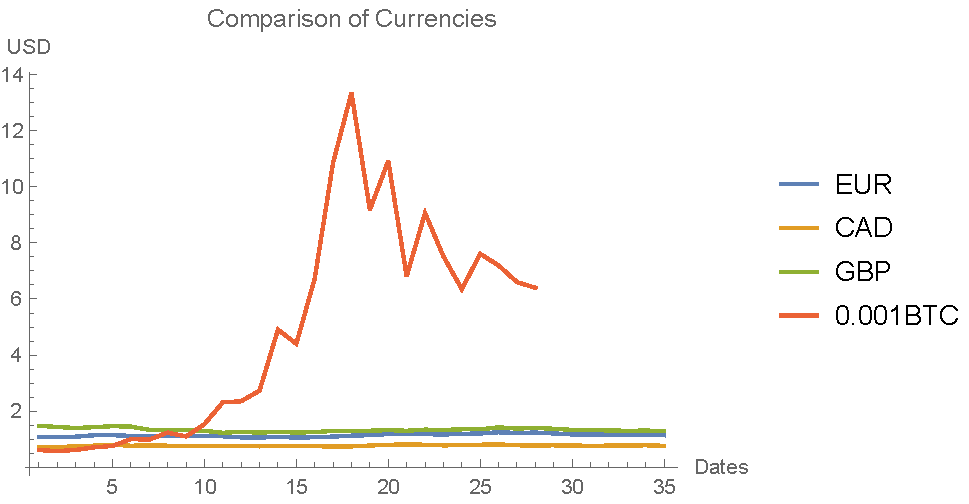
\includegraphics[width=0.75\textwidth]{figures/graph1.pdf}
	\caption{\label{fig:btcandfiat}Comparison among fiat currencies and Bitcoin: The values are retrieved on the first day of each month. A fraction of Bitcoin (1/1000 BTC) is plotted.}
\end{figure}

Figure~\ref{fig:btc} shows the change of value of Bitcoin with respect to USD and gold. The value changes happen in directions 2 and 6 (Figure~\ref{fig:legend}). The part of plot in direction 2 means that Bitcoin is gaining value against gold and USD. This can also be interpreted as both gold and USD are losing value relative to Bitcoin. %However, the first explanation is more likely to be the case, as only Bitcoin's value is changing compared to two values (USD and gold) changing.
Also, the fact that the plot is located on the diagonal shows that Bitcoin gains/loses value against both USD and Gold at the same time. This indicates that the changes in the values of USD and gold are highly correlated.

\begin{figure}[!htb]
	\centering
	\subfloat[Bitcoin's value with respect to USD and Gold]{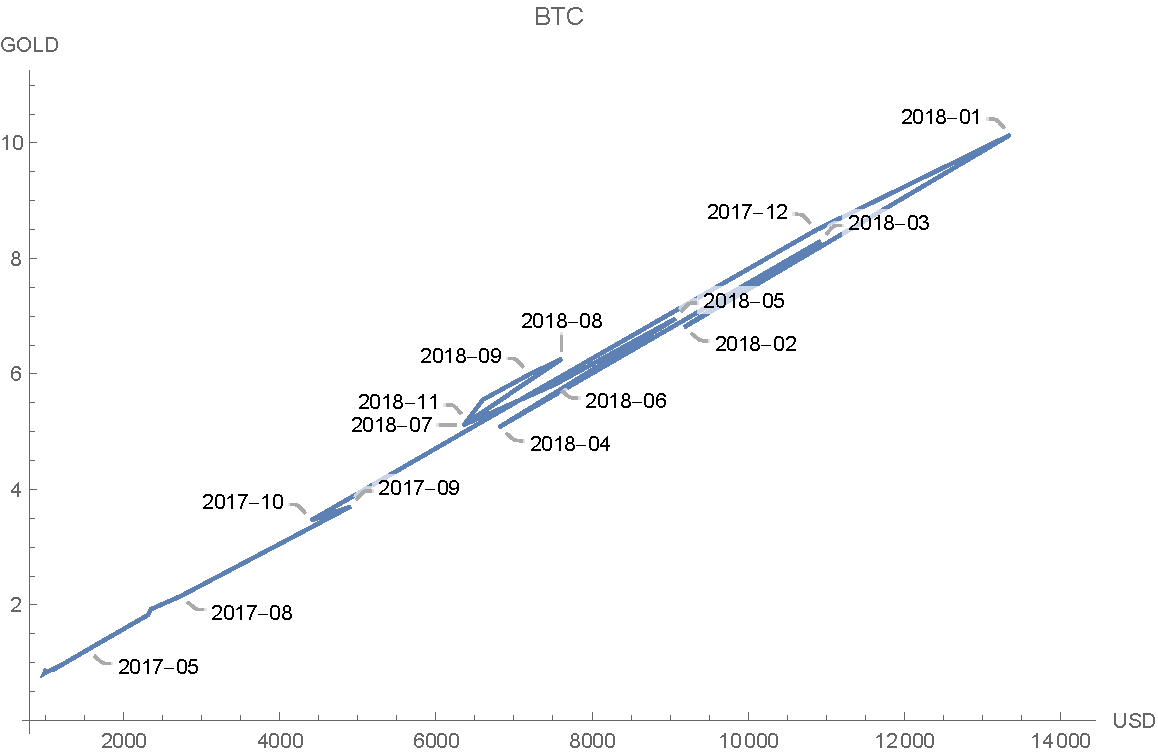
\includegraphics[width=0.75\textwidth]{figures/btc.pdf}\label{fig:btc}}
	\hfill
	\subfloat[Legend]{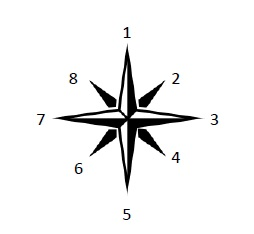
\includegraphics[width=0.25\textwidth]{figures/compass}\label{fig:legend}}
	\caption{BTC}
	\label{fig:Comparison}
\end{figure}

Considering these facts, there is a desire to design stablecoins with the stable nature of the fiat currencies together with the decentralized nature of the blockchain which is the underlying technology of cryptocurrencies.


%\begin{figure}[!htb]
%	
%	\centering
%	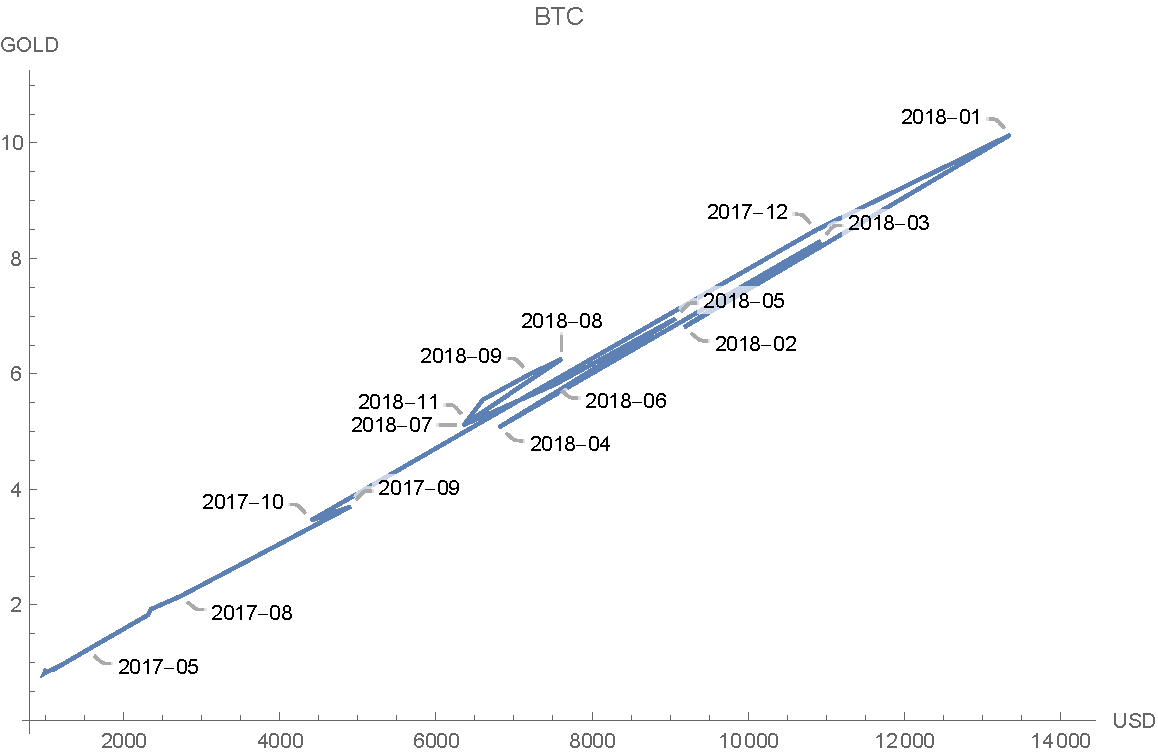
\includegraphics[width=0.65\textwidth]{figures/btc.pdf}
%	\caption{\label{fig:graph2}BTC}
%\end{figure}
%About coin supply and volatility~\cite{sams2015note}.

%~\textit{Discussion on how a stablecoin can be adopted by the majority and the comparison between other cryptocurrencies:}Rightly or wrongly, volatile cryptocurrencies like bitcoin are not viewed by many central bankers as a seriouscompetitive threat to their own national currencies. However, a stablecoin of sufficient size and use maybe deemed to pose greater direct competition to fiat currencies than bitcoin and may therefore spark a competitive response or regulatory backlash from central banks, which in many jurisdictions have largely remained on the sidelines of cryptocurrency regulation to date. What is less clear here for cryptocurrencies is “how big is too big?” Central bankers have been reluctant to provide specific quantitative levels that would trigger concerns (e.g., what percentage of payments made with a cryptocurrency would be deemed to pose a threat to a central bank’s ability to conduct monetary policy?)~\cite{report}.

%For the paper let's have a section under preliminaries and talk about what is money?where does it come from?
%useful articles for this topic:
%https://www.imf.org/external/pubs/ft/fandd/2012/09/basics.htm
%https://www.imf.org/external/pubs/ft/fandd/2010/03/basics.htm


\section{The current state of the stable coins} % Didem :

%different ways and issues with each. %~\cite{euromoney}
Stablecoins have a market value of \$3 billion and this corresponds to the 1.5\% of the total market value of the cryptoassets~\cite{report}. Each proposing different properties, stablecoins can be categorized into three groups based on the way they achieve stability: fiat-collateralized, crypto-collateralized, and non-collateralized.

~\textbf{1) Fiat-collateralized stablecoins:} These types of stablecoins are backed by fiat currency and backing by USD is one of the most common types. Generally, there is a 1:1 peg between the fiat currency and the stablecoin that indicates a convergence between their values~\cite{linkedin}. USD being one of the most common choices for the fiat currency to back the stablecoin with, IBM states that they are also interested in projects that use other national fiat currencies, as they will be helpful for IBM's blockchain integration~\cite{cointelegraph}.

Tether and TrueUSD are prominent examples of USD pegged tokens. Some projects like Digix Gold Token prefer to use gold to back their stablecoin, as gold has a relatively slow increase in its value compared to fiat currencies. %Reference??

~\textit{Discussion about centralization:} Backing up with fiat currency means that there is a need for third party. The amount of money to back the stablecoin with, should be held in an account~\cite{techrev}. Centralization ensures that the peg can be attained. However, involvement of a third party causes controversy, as the third party can just deny giving money to the users. Tether explains this point as follows~\cite{cryptoinsider}:

\begin{quote}
``Redemptions will not be unreasonably denied, but we reserve the right to selectively deny redemption and creation of Tethers on a case-by-case basis."
\end{quote}

%Globcoin: less reliance on US dollars but still centralized.~\cite{cryptoinsider}

~\textbf{2) Crypto-collateralized stablecoins:} These types of stablecoins use other cryptocurrencies as a back up value rather than a fiat currency. Over-collateralization is needed this case as the underlying cryptocurrency is also volatile~\cite{linkedin}. MakerDAO and Reserve use this approach -- utilizing a smart contract to back the stablecoin with another cryptocurrency~\cite{cointelegraph}.

If there is a black swan event~\footnote{A black swan event is characterized as being unexpected, random and having significant effects to the current situation. this type of an event is hard to predict~\cite{swan}.} where the underlying currency loses its value and does not worth anything, the stablecoin also loses its value~\cite{coinsexplained}.  Due to the over-collateralization in this type of stablecoins the loss of value will be drastic. This is the reason that a group of experts strongly discourage this approach.

~\textbf{3) Non-collateralized stablecoins:} Unlike the previous types, this group of stablecoins are not backed by fiat currencies or another cryptocurrency. Here the stability is achieved algorithmically~\cite{linkedin} which helps to provide better scalability~\cite{report}. Basis is one of the first projects that use this approach.

Basis and Carbon use the dual-token model~\cite{cryptoinsider}. ~\textblue{Is the following sentence explaining the approach used in Basis or Carbon, if not let's bring them up}There is dynamic adjustment of the existing supply of the stablecoin. While one token is stable, the other is used to achieve the stability of the value. If the value of Basis increases (an increase over \$1), more Basis tokens are produced to increase the supply which will lead to a decrease in the price and if there is a decrease in the price, a bond that is worth a Basis token is issued and some Basis tokens are bought to decrease the supply.~\cite{euromoney}

%If the price falls below \$1, the code will issue bonds worth one basis token each, use the proceeds to buy existing Basis tokens to reduce supply and so bid the price back up, later repaying bondholders when Basis tokens trade above par.  It is a complicated, seigniorage based system.

%The dual-token model — stablecoins and shares One token is stable, and the other is used to whip it back onto the narrow track. Roughly, the idea is that supply of the stable token is dynamically increased and decreased. ex: Basis, Carbon. Then the dual-token model has two flavours: the kind where the stable token is created by locking up other crypto (e.g. DAI and Havven), and the kind where it is not (e.g. Basis, Carbon). ~\cite{cryptoinsider}  DAI Havven crypto collat?
~\textblue{seigniorage shares method is the one to achieve stablecoin?}
Another approach is the seigniorage shares method\cite{overview}. Here, the smart contract automatically adjusts the supply based on the algorithm to achieve stability in the value.

\section{Issues that stablecoins address}
As mentioned in the~\ref{Intro}, currencies have to serve as a store of value, a unit of account, and a medium of exchange~\cite{smithin2002money}. To do so, they have to denote a minimum level of value stability. In this regard, stablecoins are proposed to fulfill these properties, due to their non-fluctuating value compared to fiat currencies or any other alternative\eg commodity. In addition, they purport to solve a group of critical issues that were introduced by cryptocurrencies. In this section, we discuss these issues.

\subsection{Cryptocurrencies as Medium of Exchange}
Despite the fast growth of the cryptocurrencies and decentral applications, there is still little deployment of them in the daily payment procedures of businesses. The main reason is that these assets are volatile in the price and hence highly risky to be deployed by merchants and retailers \ie it is impossible for a company employer to provide the employees' incomes in a volatile cryptocurrency \eg BTC that has a high level of future value and price uncertainty. On the other hand, having a stable price over the time, stablecoins can serve as a true medium of exchange, while they preserve all the advantages of using cryptocurrencies as opposed to fiat currencies.

\subsection{Cryptocurrencies as Unit of Account}
Money has to serve also as a unit of account-- the common measure that sets price to goods and services. Fiat currencies \eg USD, EUR \etc serve this functionality correctly, so they are used as units of account in the US and Europe respectively. Unfortunately, cryptocurrencies such as BTC, not having a stable price, do not seem to be used as a unit of account, hence will not be able to serve as money. However, given the price stability that stablecoins offer, they have a higher chance to be used as a digital representation of a unit of account.

\subsection{Cryptocurrencies as Store of Value}
Any asset, commodity, or money that maintains its value is called a store of value. As mentioned in Section~\ref{Intro}, highly volatile cryptocurrencies (\ie Bitcoin) cannot fulfill this property of money, as they cannot maintain their purchasing value for long-term. In contrast, stablecoins can be accepted as a store of value as their price remains stable over the time.

%\subsection{dApps}
%from the blockchain paper:
%In the web 3.0 stack, decentralized applications (?dApps?) are being built on top of infrastructure protocol
%layers. Many of those applications will likely rely on price stable cryptocurrencies to distribute value.
%Stablecoins should accelerate the shift from token speculation to usage in dApps as users won?t be
%incentivised to hold (or sell) the token in anticipation of future price appreciation (or depreciation). This
%should in turn increase the token velocity and fulfil the potential of decentralised networks.
%dApps are the channel through which stablecoins are likely to be brought to the masses in the foreseeable
%future. For example, MakerDAO and Dether recently partnered to bring Dai to mobile ATMs.
%Finally, ERC20 stablecoins can be held and transferred by anyone who already has an Ethereum wallet, and nearly half of all stablecoin projects (48\%) are running on Ethereum. Provided that Ethereum is a successful underlying infrastructure protocol for dApps, ERC20 stablecoins should be adopted faster and benefit from the Ethereum vibrant ecosystem.

\subsection{Lending with Cryptocurrencies}
Despite quite a few blockchain applications in financial technologies, there has been little deployment of lending.
Lending is difficult to be deployed on the blockchains, bdue to the monetary instability observed in the existing cryptocurrencies~\cite{okoyetoward}. This volatility has led the cryptocurrencies to be used more as speculative investments instead of serving as store of value and unit of account. In a lending situation with volatile currencies, where their values are being depreciated or appreciated over time, the cash taker will eventually owe more than what he has borrowed or the vice versa. Therefore, the volatility in the value of cryptocurrencies causes serious concerns and difficulties both for cash takers and cash providers~\cite{okoyetoward}. In contrast, lending perfectly works if a loan is done with a stable cryptocurrency, whose value remains stable over the time.

%\subsection{Government Surveillance}
%
%Governments have recently started examining  the idea of issuing a central bank-issued digital currency (CBDC)~\cite{barrdear2016macroeconomics}. These national digital currencies are regulated by federal regulators instead of serving in a form of decentralized currencies-- where only the owner has the sole control and ownership of the assets. CBDCs are not backed by any tangible assets and are issued by central banks so that they could keep their monetary policy while adopting the trend of digital assets. However, an oppressive government may abuse these assets to manipulate the markets or to limit the ownership of these assets to  a special group of people (\eg citizens of that specific country). However, since stable coins are not backed by any central party and financial regulator, users are assured about the stability as well as having easier access no matter where they live and/or come from.

\subsection{Remittance}

Although cryptocurrencies, especially Bitcoin, play a revolutionary role in financial systems, they are yet not easy to transact with due to their volatile characteristics. Therefore with stablecoins, one can benefit from decentralized nature of the token, while there is no price volatility risk. In addition, stablecoins make the cross border payments, remittances, easier.


% nation issued digital assets can be
%
%After all, fiat currencies are not backed by any tangible assets. You can?t return the currency to the government in exchange for a bar of gold or silver, a can of beans, a pack of cigarettes, or any other items that might have value to you. Fiat currencies are backed by the full faith and credit of the government that issued them and nothing more. If you want gold, silver, beans, or smokes you need to exchange your fiat currency with a person or entity that possesses the item that you want.
%
%Read more: Why Governments Are Afraid of Bitcoin | Investopedia https://www.investopedia.com/articles/forex/042015/why-governments-are-afraid-bitcoin.asp#ixzz5VLsy6DKS
%Follow us: Investopedia on Facebook
%
%
%The reason is tha due tokeep their monetary poli and power.
%
%
%
%
%The concept of CBDCs, or national digital currencies ? the scenario in which the trend of digital currencies gets adopted by a federal regulator, essentially under its rules, with the central bank issuing digital fiat money, rather than cryptocurrencies in their most popular, decentralized form and becomes not only a regulator, but clients? account holder as well ? has attracted many governments across the world. Some of them have already implemented the idea, some keep researching, while others ? like Germany ? have dismissed the idea altogether. Here?s a list of those countries along with their reasonings for/against CBDCs.
%
%
%For the most avid supporters of digital currencies like Bitcoin, the idea of having a central banking system goes against everything they believe. After all, Bitcoin was created as a means for people to ditch the banking system and allow them the freedom to handle their own financial affairs.
%
%The most pressing reason for a government to launch a cryptocurrency is the success of private cryptocurrencies. This isn?t out of some misplaced sense of competition, but rather because governments would be loathe to lose control of their nation?s monetary policy. When asked about the potential governmental response to cryptocurrencies, former IMF Chief Economist Kenneth Rogoff?s response was, ?When it comes to the monetary system, the government makes the rules. You cannot win the game. If they're not winning, they will change the rules.? If this doesn?t mean stringent regulations?and governments so far have been much more concerned about the scammy or bubbly elements of the crypto world than its capacity for toppling fiat?it could mean govtcoins.
%
%
%Stablecoins carry several advantages over govtcoins. For one, since stablecoins are not ?issued? by nation states, users do not have to worry about government surveillance. In countries helmed by oppressive governments, decentralized stablecoins could still be popular for this reason.
%
%
% Additionally, it?s reasonable to project that if governments can program their currencies, taxes will be built into the govtcoin. If people or entities wish to avoid taxes, they could choose to stash their capital in decentralized stablecoins over currency havens or other govtcoins (though this is obviously not recommended - ?always pay your doctor and the IRS?).
%
%
%Finally, stablecoins also offer potentially easier access as governments might attempt to restrict ownership of their cryptocurrencies to own-country citizens.



%https://www.bis.org/cpmi/publ/d174.pdf
%https://www.bankofcanada.ca/wp-content/uploads/2017/11/sdp2017-16.pdf


%\subsection{Promoting Trust in the Crypto Space}
%Discussion on Paxos, Gemini vs Tether. How having monthly attestations increase the reliability of Paxos and Gemini?
%
%For a stablecoin to consistently trade at par, its issuer must, in effect, convince a wide a community of future tokenholders of its future solvency. And that degree of trust can be hard to maintain, as it involves the psychology of the market, which can shift significantly over time.
%Consider Tether's predicament. Whether it has the funds it says it has isn't the only question. The other, perhaps even more important, is whether the market believes those commitments will hold up against a wider environment of waning confidence.
%
%For reserves-backed stablecoins, this includes practices such as: naming the banking relationship so that users can properly assess the underlying counterparty risk; committing to independent security audits of the underlying code to show that tokens are destroyed when funds are redeemed; holding regular attestations of the firms' balances by trusted third-party auditors. (Note: this does not mean a full "audit" per se. Calls for an audit of Tether were misleading; there is no way that a crypto system's past transactions can be audited in the traditional sense. Instead, proofs rely on attestations as to the accuracy of the firm's claims about its balances at a point in time.)
%
%(https://www.coindesk.com/the-delicate-psychology-of-stablecoins/)

%to be completed >> @Mahsa

%their value is designed not to fluctuate
%
%
%
%Trust: In addition to fostering trust in cryptocurrencies, the other main aim of the Gemini dollar is to promote the use of coins that operate on blockchain. Right now, the main reason people put money in cryptocurrencies is to make more money. ?When something is a store of value, you generally don?t want to spend it,? Tyler Winklevoss told Business Insider. With stablecoins, there?s no money-making incentive. People who buy them will do so presumably for the unique advantages transacting with cryptocurrencies provides, like seamlessly (and fee-lessly) sending money overseas.
%
%
%
%https://medium.com/@usdx/five-issues-confronting-stablecoins-for-the-rest-of-2018-75245820fdb5

%\subsection{Smart Insurance}
%combine programmability + stability > when the flight gets cancelled or delayed the smart contract will \textbf{automatically} pay the passengers. In this situation, an stable coin is needed.
%from the blockchain report: In travel and many other smart insurance use cases, it would be preferable to denominate the smart contract with a stablecoin rather than a more volatile cryptocurrency, such as ether (ETH). Generally, people take out insurance to reduce risk and would therefore want smart contract insurance underpinned by a stable currency.

%\textit{Other possible solutions to lending:} ~\textblue{While stable coin is one of them what can be the other possible solutions?}
%
%\textblue{Taken from ~\cite{okoyetoward}, paraphrasing needed!}
%Addressing monetary instability:
%\begin{itemize}
%	\item The rate of release of new currency into the system could be modified to en-
%	able new currency to be introduced at (i) a more insightful rate or (ii) based
%	on some internal metrics of the system like number of transactions. [Remark:
%	an insightful rate has been elusive despite many alt-coins customizing the
%	schedule and it is difficult to see how metrics could not be gamed].
%	\item A cryptocurrency can also use explicit pegging but it is no better suited to this system than standard currencies.
%	\item A central bank could manage currency circulation while allowing other as-
%	pects to be decentralized. [	Remark:Central banks have been historically
%	unsuccessful at using money circulation as a target].
%	\item The loan could be use the cryptocurrency as the medium of exchange but
%	use a stable (e.g.,	government) currency as the unit of account.
%\end{itemize}
%
%\textit{Other possible solutions to lending:} While stable coin is one of them what can be the other possible solutions?

%\section{Comparison Framework} % Put the code for the framework
%Define the properties that are considered during the design of stable coins.
%~\textblue{Collateralization info from ~\cite{bitmex}, decide which projects to choose that exemplify each category best.}
%\begin{table}[]
%	\begin{tabular}{|l|l|l|l|l|}
%		\hline
%		& Collateralization  & Price Oracle & Centralization & Feedback Mechanism
%		\\ &(+ the value of the collateral)&&&
%		 \\ \hline
%		BitShares (BitUSD) &  Crypto-collateralized &  & &\\ \hline
%		BitBay & Non-collateralized & & & \\ \hline
%		 DAI& Crypto-collateralized (ETH)  &  Yes& No & Target Price, Target rate,\\
%		 &&&&Sensitivity Parameter,\\
%		 &&&&Global Settlement \\ \hline
%		 Basis&Non-collateralized&& &\\ \hline
%		 Tether & Fiat-collateralized (USD) & & Yes &\\ \hline
%		  &&&& \\ \hline
%	\end{tabular}
%\end{table}

%Decentral price oracle and Schelling point~\cite{cryptoinsider}
%DAI and Bitshares~\cite{cryptoinsider}
%Feedback column from ~\cite{report}
%Bitbay: One of the most unstable stablecoins~\cite{report}.

%Today, it would appear that prioritization of automation/transparency generally carries with it the trade-off of greater stability complexity (i.e., risk that the peg will be broken). In other words, the more decentralized the stablecoin design, the less likely it is to remain price stable against a peg like the US dollar. The success of Tether offers at least some evidence that so far the market has prioritized stability overdecentralization (i.e., transparency and automation).Anyone who prioritizesdecentralization already has the option to own arguably the most decentralized cryptoasset, bitcoin.~\cite{report}
%~\textit{A question to think about: }But does the broader world beyond the digital assets ecosystem really need (or want) stablecoins?~\cite{report}
% Tether, the largest stablecoin in terms of its market value of approximately $2.7 billion USD, illustrates the underlying demand for a stablecoin

\section{Investigation of gas volatility in Ethereum}
\begin{figure}[!htb]
	\centering
	\subfloat[EUR]{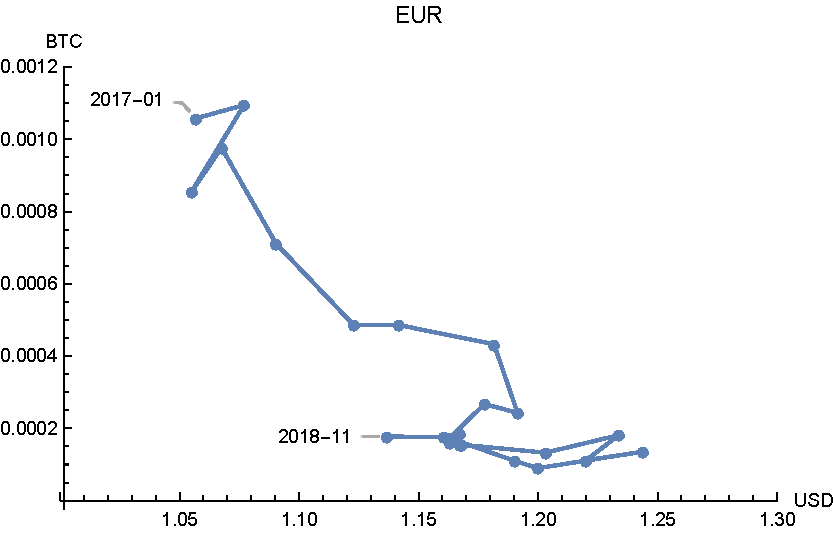
\includegraphics[width=0.5\textwidth]{figures/eur.pdf}\label{fig:eur}}
	\hfill
	\subfloat[ETH]{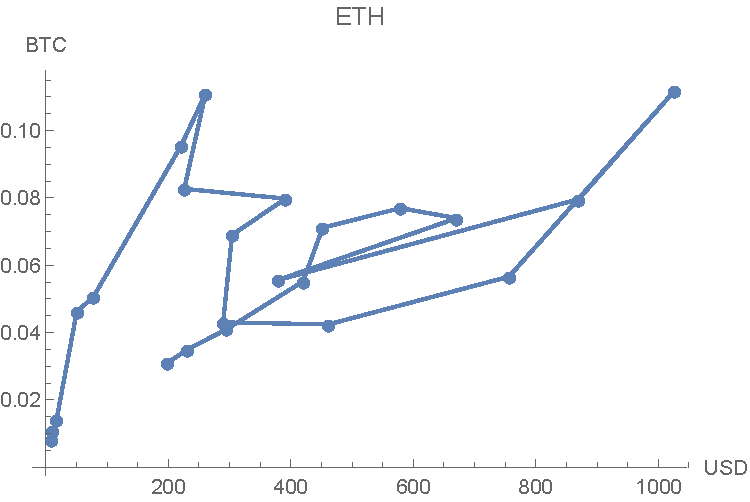
\includegraphics[width=0.5\textwidth]{figures/eth.pdf}\label{fig:eth}}
	\hfill
	\subfloat[GAS]{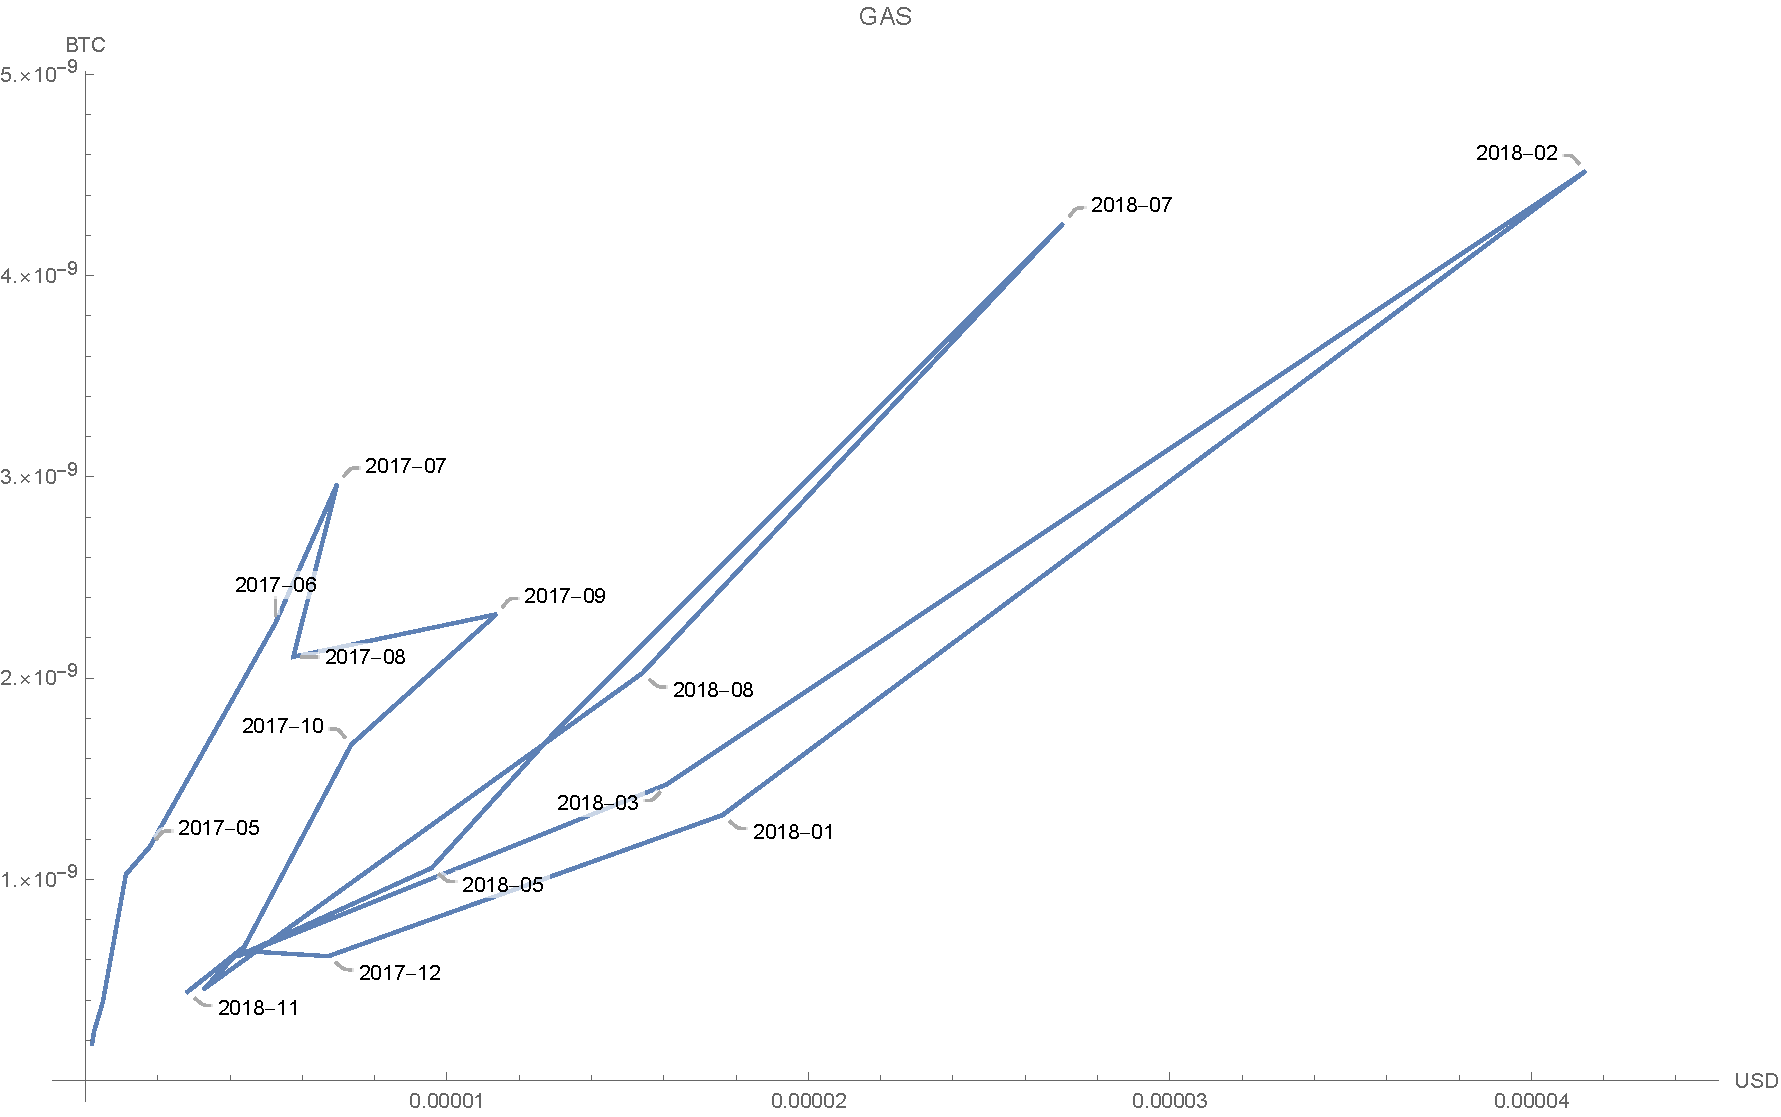
\includegraphics[width=0.5\textwidth]{figures/gas.pdf}\label{fig:gas}}
	\hfill
	%\subfloat[Gold]{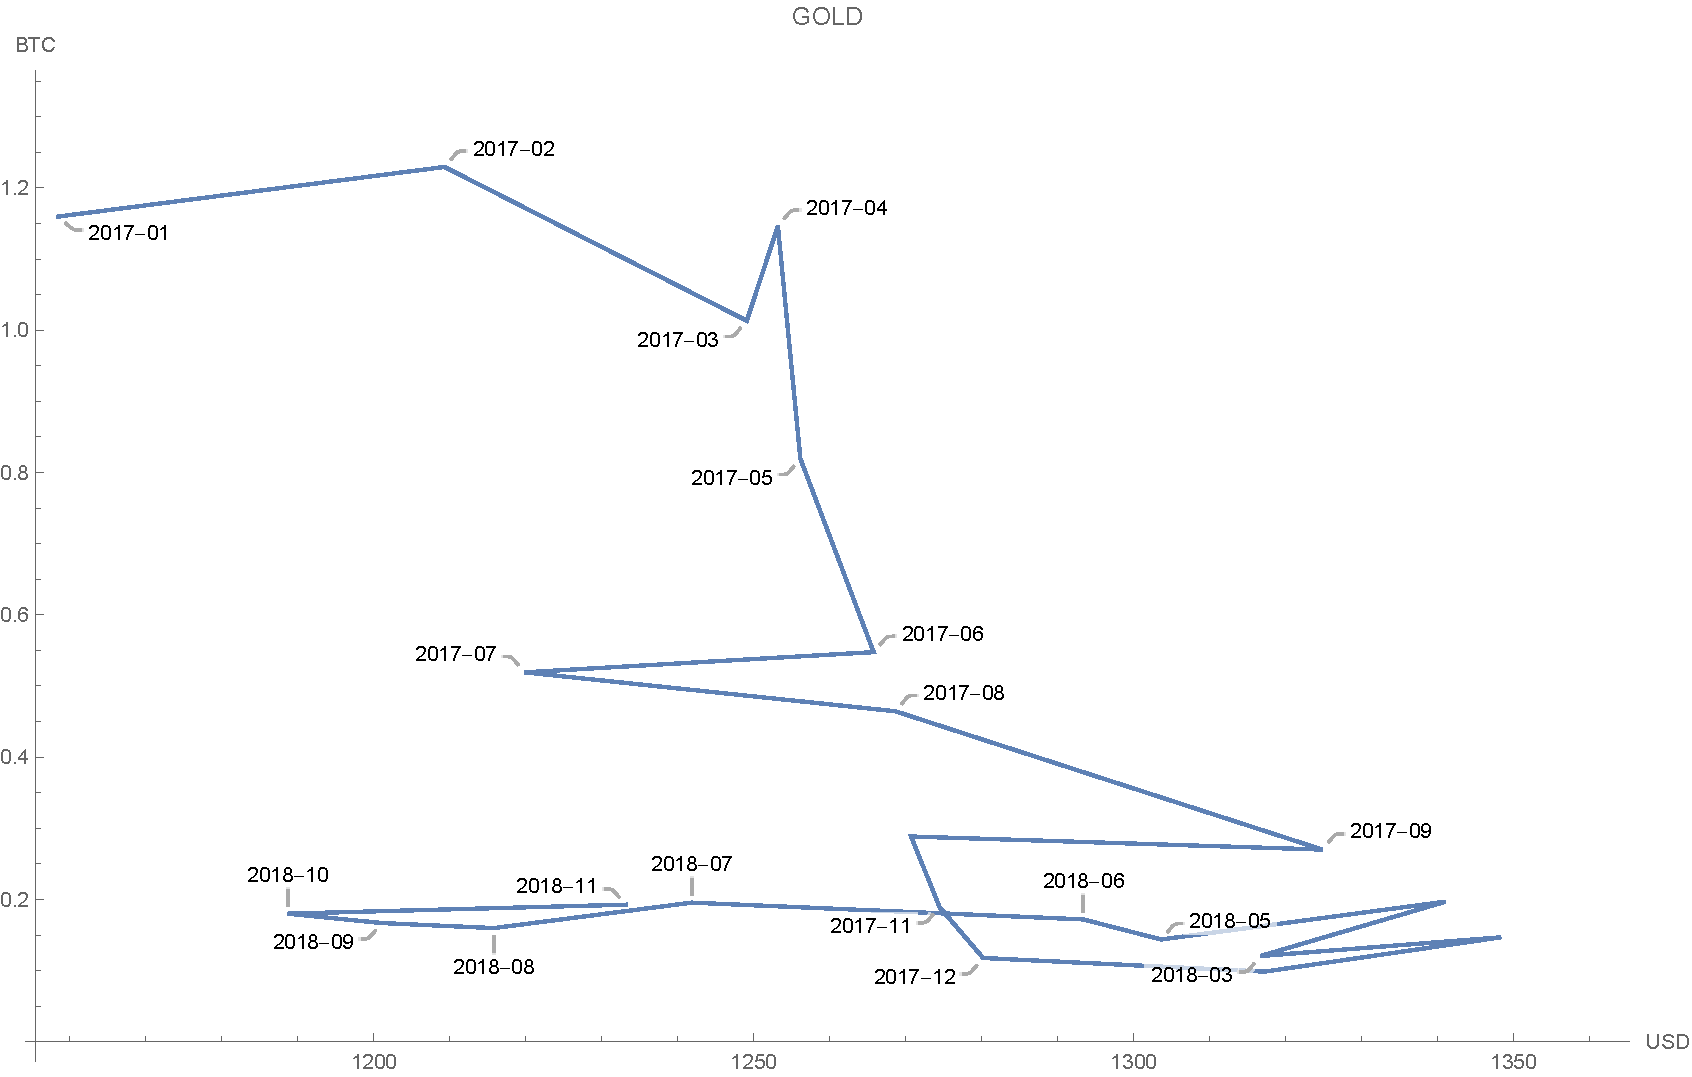
\includegraphics[width=0.5\textwidth]{figures/gold.pdf}\label{fig:gold}}
	\caption{Comparison of change of value in EUR, ETH and Gas with respect to gold and BTC }
	\label{fig:aboutgas}
\end{figure}

Figure~\ref{fig:aboutgas} illustrates how the values of EUR, ETH and Gas change with respect to BTC and gold. EUR plot in Figure~\ref{fig:eur} tends to have more movements in the directions 1-5 and 3-7 suggesting that while the value of EUR stays the same according to one axis, it changes according to the other. For instance, between June 2018 and August 2018, the value of EUR increased with respect to BTC, while it stayed the same according to USD. This type of movement suggests that EUR-USD exchange rate is going under less change, whereas BTC-EUR rate is subject to high volatility. On the other hand, in the first half of 2017, while EUR retained its value against BTC, EUR to USD rate went under change.

ETH plot in Figure~\ref{fig:eth} illustrates more volatility against BTC and gold, as there are horizontal, vertical and diagonal changes. The fact that the points are spread in a large range of values indicates drastic changes in ETH price with respect to BTC, which is also a volatile cryptocurrency, and Gold.

Compared to Figure~\ref{fig:eur} and Figure~\ref{fig:eth}, gas plot (Figure~\ref{fig:gas}) has mostly diagonal changes, spread over a smaller range. There are less number of changes compared to ETH. Except from the changes between May 2018-July 2018 and January 2018-March 2018, the gas price changes in a smaller range. Even though there are fluctuations in the gas price, it can be inferred that gas price is less volatile than ETH.

\section{Conclusion and Discussion}
In this paper, we analyze the current state of stablecoins with the various options that have been so far proposed to achieve price stability. We also discuss various issues that if the righteousness stablecoins are designed, would address them. According to the charts represented in the paper, we hypothesize there are two options to achieve stablecoin, that is, pegging the stablecoin to a (i) currency (\ie USD) or (ii) commodity (\ie gold). In the first case, 






This report analyses the current state of stablecoins and investigates the gas price in Ethereum to understand how gas price behaves. Stablecoins have a high a potential to offer a wide range of applications due to their price stability.

%\section{Critical Issues with Stable Coins}
%~\textblue{Combine with conclusion and discussion??}
%
%--Most stable coins fail (this is historically true, it doesn?t speak to the current stable coins). When they fail, they may or may not be redeemable for the promised amount. That is the harsh truth. None of the old stable coins are with us today aside from Nubits?. and Nubits has recently been trading for under .50 cents here in late March 2018. TUSD, Tether, and Dia all seem solid in there here and now, and they likely have learned from the mistakes of their formers, but if we are being honest about the history of stable coins, it is as volatile as the history of crypto itself.
%
%--Some say that stable coins bring stability to the crypto space, but that idea doesn?t seem to be empirically proven. Instead, I?d argue that the perks of stable coins are in the ability for traders to go to a dollar quickly and the ability of exchanges to increase liquidity. Further, I?d argue that stable coins actually add volatility to the crypto space, because they allow for more speculation (which in theory creates stability, but which in practice hasn?t really seemed to do anything of the sort). The bottom line on this point is that the crypto space isn?t a stable place, and no type of cryptocurrency, regulation, or derivative I?ve seen has yet to change that (so here the point is, let us not give credit where it is not due). The term used is ?stable coin? or ?price-stable cryptocurrency,? not because this coin brings stability, but because the token ideally holds a stable value.
%
%--Stable coins generally require us to trust a central third party. Each stable coin has its own way around being overly centralized, but there generally needs to be some way to manage these assets to ensure their stability (even though they tend to be blockchain based). Anything centralized requires the trust of a third party to some extent. Requiring the trust of a third party in crypto goes against the concept of crypto somewhat. This isn?t a problem per-say, but it is worth noting. With that said, most exchanges aren?t decentralized and thus using a stable coin as a currency on an already centralized exchange is hardly the a reason not to use stable coins (or exchanges).
%
%-Discussion about collateralization: The second type of stable coin is partly collateralized. In this case, the platform holds dollars equal to, say 50\%, of the value of the coins in circulation.The problem with this variant will be familiar to any monetary policy maker whose central bank has sought to peg an exchange rate while holding reserves that are only a fraction of its liabilities.
%If some coin owners harbor doubts about the durability of the peg, they will sell their holdings. The platform will have to purchase them using its dollar reserves to keep their price from falling. But, because the stock of dollar reserves is limited, other investors will scramble to get out before the cupboard is bare. The result will be the equivalent of a bank run, leading to the collapse of the peg.
%
%--A discussion about the price comparisons between the stablecoins  https://www.coindesk.com/which-stablecoin-is-the-riskiest-the-crypto-market-is-pricing-that-in/
%
%--speculative attacks on pegged exchange rates https://www.marketwatch.com/story/your-crypto-stable-coin-isnt-tethered-to-anything-2018-09-12
%
%--Ametrano's paper on currency design (the one that inspired Fragments) argues that we shouldn't peg a stablecoin to the U.S. dollar, as its days of stability may be numbered. Ametrano's preferred benchmark is a basket of commodities. ~\cite{cryptoinsider}

%%https://gemini.com/wp-content/themes/gemini/assets/img/dollar/gemini-dollar-whitepaper.pdf -> ref

%Mahsa:
%Other stability benchmarks besides the US dollar are also being employed by stablecoins, including baskets of various fiat currencies (e.g., IMF Special Drawing Rights), commodities or other tangible assets (e.g., gold, real estate), or economic measures (e.g., indexed inflation).
%stable coins have inbuilt mechanism to minimize exchange rate volatility.
%Another important point to emphasize is that stablecoins are simply price-stabilized cryptocurrencies, meaning they incorporate many of bitcoin or ether?s most compelling features: programmability (e.g., smart contract integration), efficiency (e.g., low-to-zero transaction fees, fast settlement times), fungibility, open (i.e., permissionless) access, and so on.
%Market makers and traders may also welcome the steadier nature of stablecoins as they carry out their daily operations.
